\documentclass[Thesis.tex]{subfiles}
\begin{document}

\chapter{Examples}

\section{Branched coverings of $\Chat$}
In this section we discuss Riemann surfaces that arise as branched double coverings of $\hat{\C}$. A Riemann surface that can be represented as a double cover of $\Chat$ is called elliptic for $g=1$ and hyperelliptic for $g>1$~\cite[p.~235]{Jost2007}. Such a double cover of $\Chat$ can be described by the
set of solutions of an algebraic equation.

\begin{definition}
Let $\lambda_1,\ldots,\lambda_{2g+2}\in \hat{\C}$, $\lambda_i\neq \lambda_j \forall i\neq j$. The
set

\begin{equation}
\label{eq:branched_cover}
C=\{(z, \mu)\in\C^2 \mid \mu^2 = \prod_{i=1}^{2g+2}(z-\lambda_i)\}
\end{equation}

is called an \emph{algebraic curve of genus $g$}.
\end{definition}

$C$ is a one dimensional complex manifold. The projection $\pi:C\to\Chat$, $C\ni(z,\mu)\mapsto z$ is a branched double cover of $\Chat$. The points $\lambda_1,\ldots,\lambda_{2g+2}\in \hat{\C}$ are called
the branch points of $C$.

In order to discretize this construction and uniformize the corresponding discrete Riemann surfaces
we need a notion of discrete double cover of $\Chat$.

\begin{definition}
Let $C$ be an algebraic curve of genus $g$. Let $V = \{\lambda_1,\ldots,\lambda_{2g+2}\}$ be the set of
branch points of $C$. A triangulation of $\pi(C)$ with vertices $V$ is called a discrete double cover of 
$\Chat$.
\end{definition}

Note that by stereographic projection the triangle mesh of the discrete Riemann sphere is projected to a
discretely conformally equivalent triangle mesh, see Theorem~\ref{thm:moebius_invariance}.

\begin{definition}
Let $S$ be a discrete surface without boundary and vertices $v_1,\ldots,v_n\in\S^2$. $S$ is a \emph{discrete double branched cover} if there exist $i_1,\ldots, i_{2g+2}\in \N$ such that ... \marginpar{complete definition}
Let $\Chat_V$ be the discrete Riemann sphere with vertex set $V\subset S^2$. Let $v_1,
\ldots,v_{2g+2} \in V$ for $g\in \N$. A \emph{discrete double cover} of $\Chat_V$ 
\end{definition}

A discrete branched cover of $\Chat$ is a triangulation of $\pi(C)$ with vertices at $\lambda_i$.


\subsection{Elliptic curves}

Let $C$ be an elliptic algebraic curve and $R$ the corresponding Riemann surface. Let $\lambda_1, \ldots, \lambda_4 \in \Chat$ be the branch points of $C$. 

\begin{example}
The most natural (and simple) example of a discrete elliptic curve is generated by the regular tetrahedron
\begin{equation}
	\mu^2=z(z^3-1)
\end{equation}

\end{example}

\begin{figure}[p]
	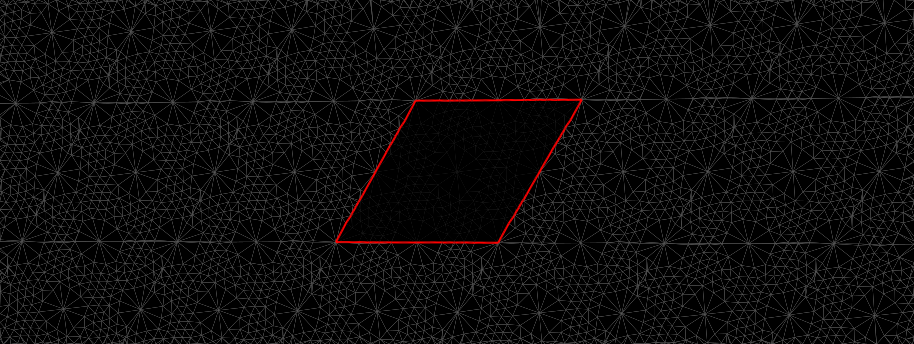
\includegraphics[width=\textwidth]{elliptic_curves/tetrahedron}
	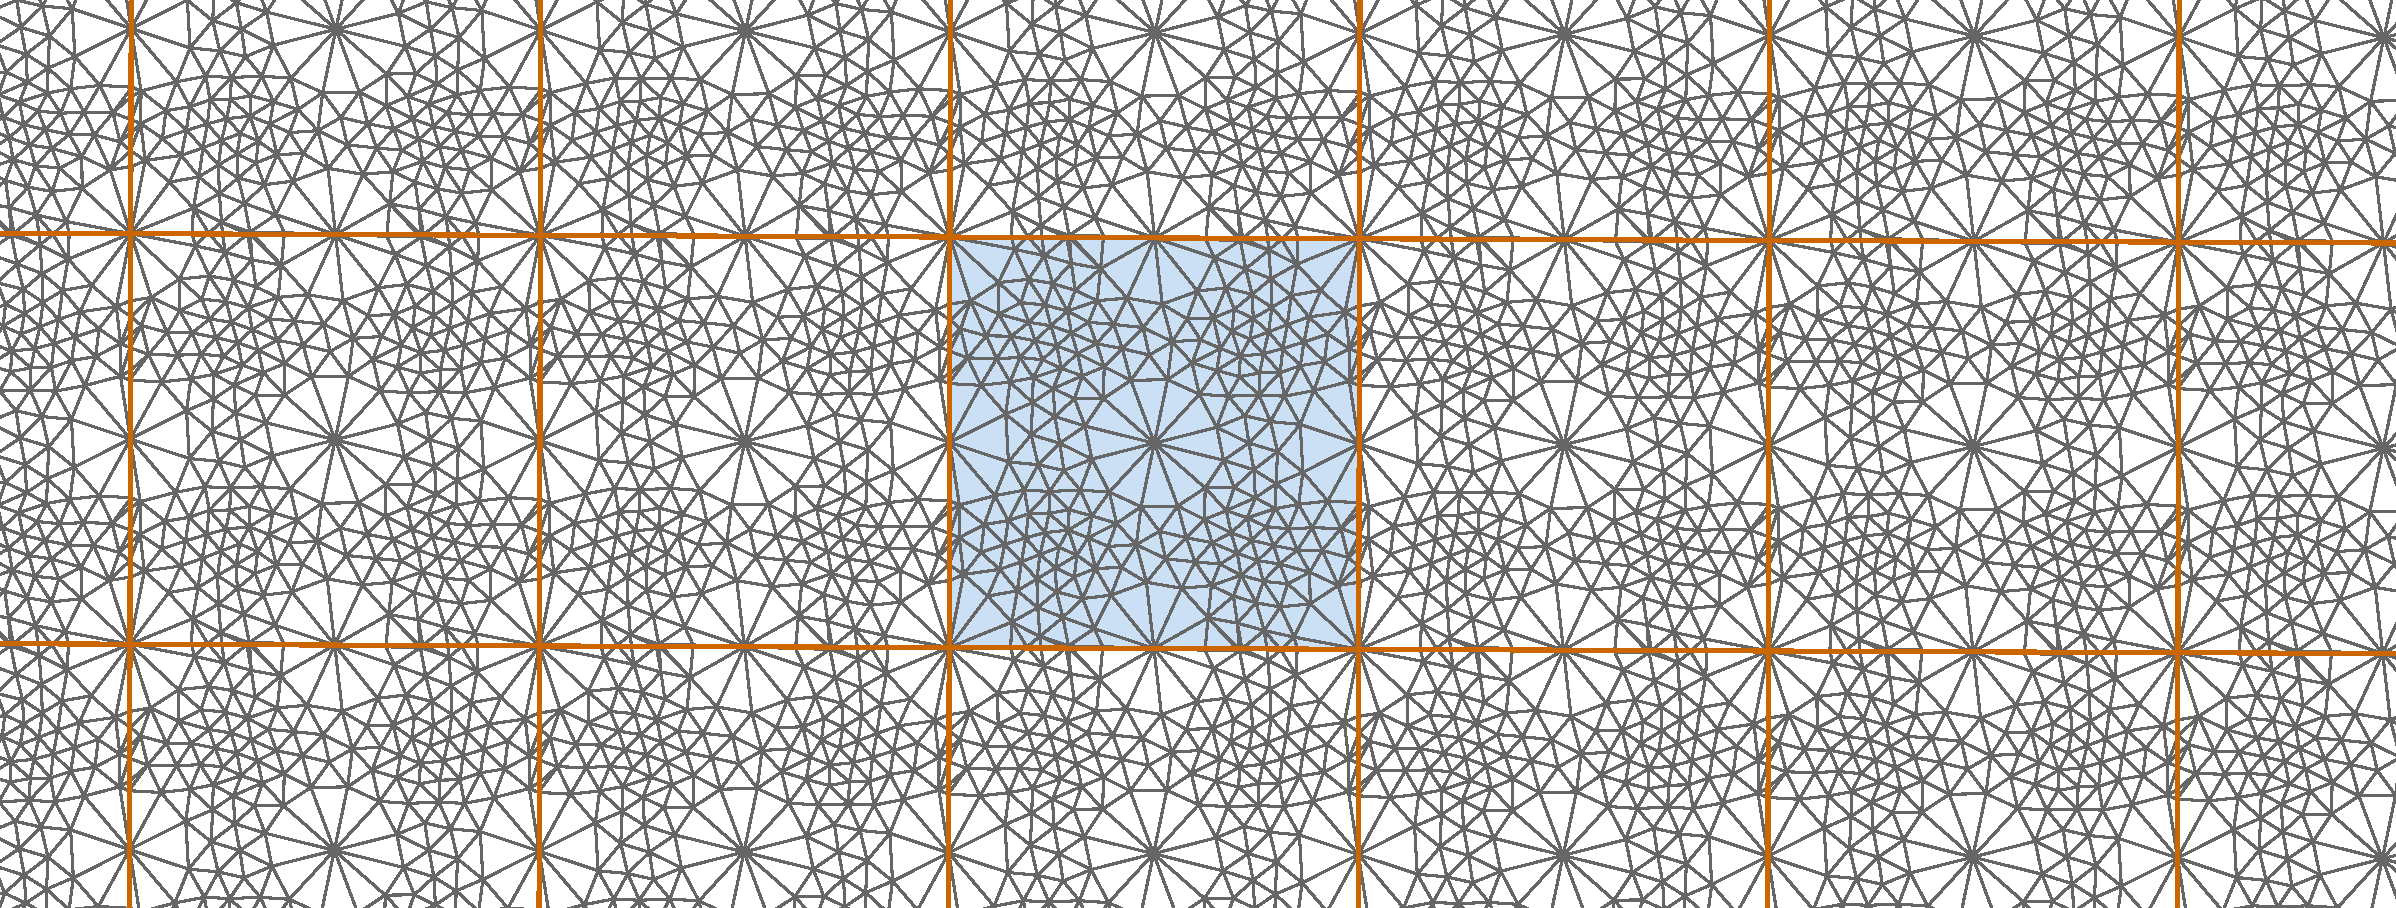
\includegraphics[width=\textwidth]{elliptic_curves/square}
	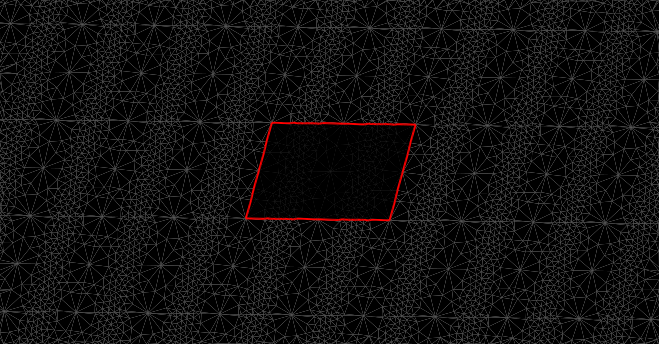
\includegraphics[width=\textwidth]{elliptic_curves/generic}
	\caption{Discrete Weierstrass $\wp$ functions. Regular tetrahedron (top), Square
	(middle), generic position branch points.}
\end{figure}

\subsection{The moduli space}
\subsection{Numerical convergence analysis}

\subsection{Construction of hyperelliptic surfaces}

\begin{definition}
	A Rielmann surface is called \emph{hyperelliptic} if it admits a two-sheeted holomorphic map to
$\Chat$.
\end{definition}

Any hyperelliptic Riemann surface can be expressed as an algebraic curve of the form
\[ w^2 = \prod_{i=1}^{2g+2}(z-\lambda_i) \quad\quad g\geq1,\quad \lambda_i\neq \lambda_j \forall i\neq j.\]
Here $\lambda_i$ are the branch points of the doubly covered Riemann sphere.

\begin{example}
The surface 
\begin{equation}
	\label{eq:regular_hyperelliptic}
	\mu^2=z(z^6-1)
\end{equation} 
is a genus $3$ surface with $6$ branch points at the 
roots of unity and at zero and at infinity. This surface admits a regular fundamental polygon.
The cuts on the surface to create a regular polygon are shown in Figure~\ref{fig:regular_branchdata}.
\end{example}

\begin{figure}[h]
\centering
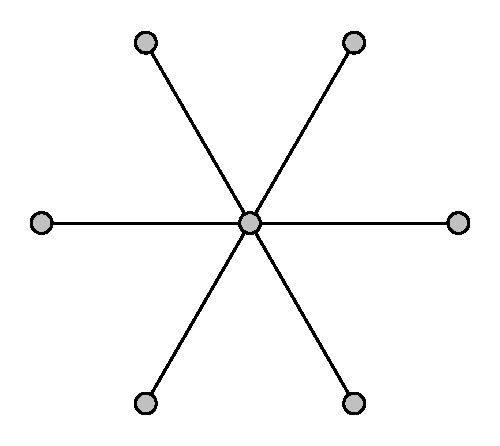
\includegraphics[width=0.2\linewidth]{data/g3_hyperelliptic01/curve.pdf}
\caption{Branch (grey) points and cuts (black lines) of the surface~\ref{eq:regular_hyperelliptic}.
Figure~\ref{fig:regular_cover} shows the uniformization of this surface.}
\label{fig:regular_branchdata}
\end{figure}

\begin{figure}
\centering
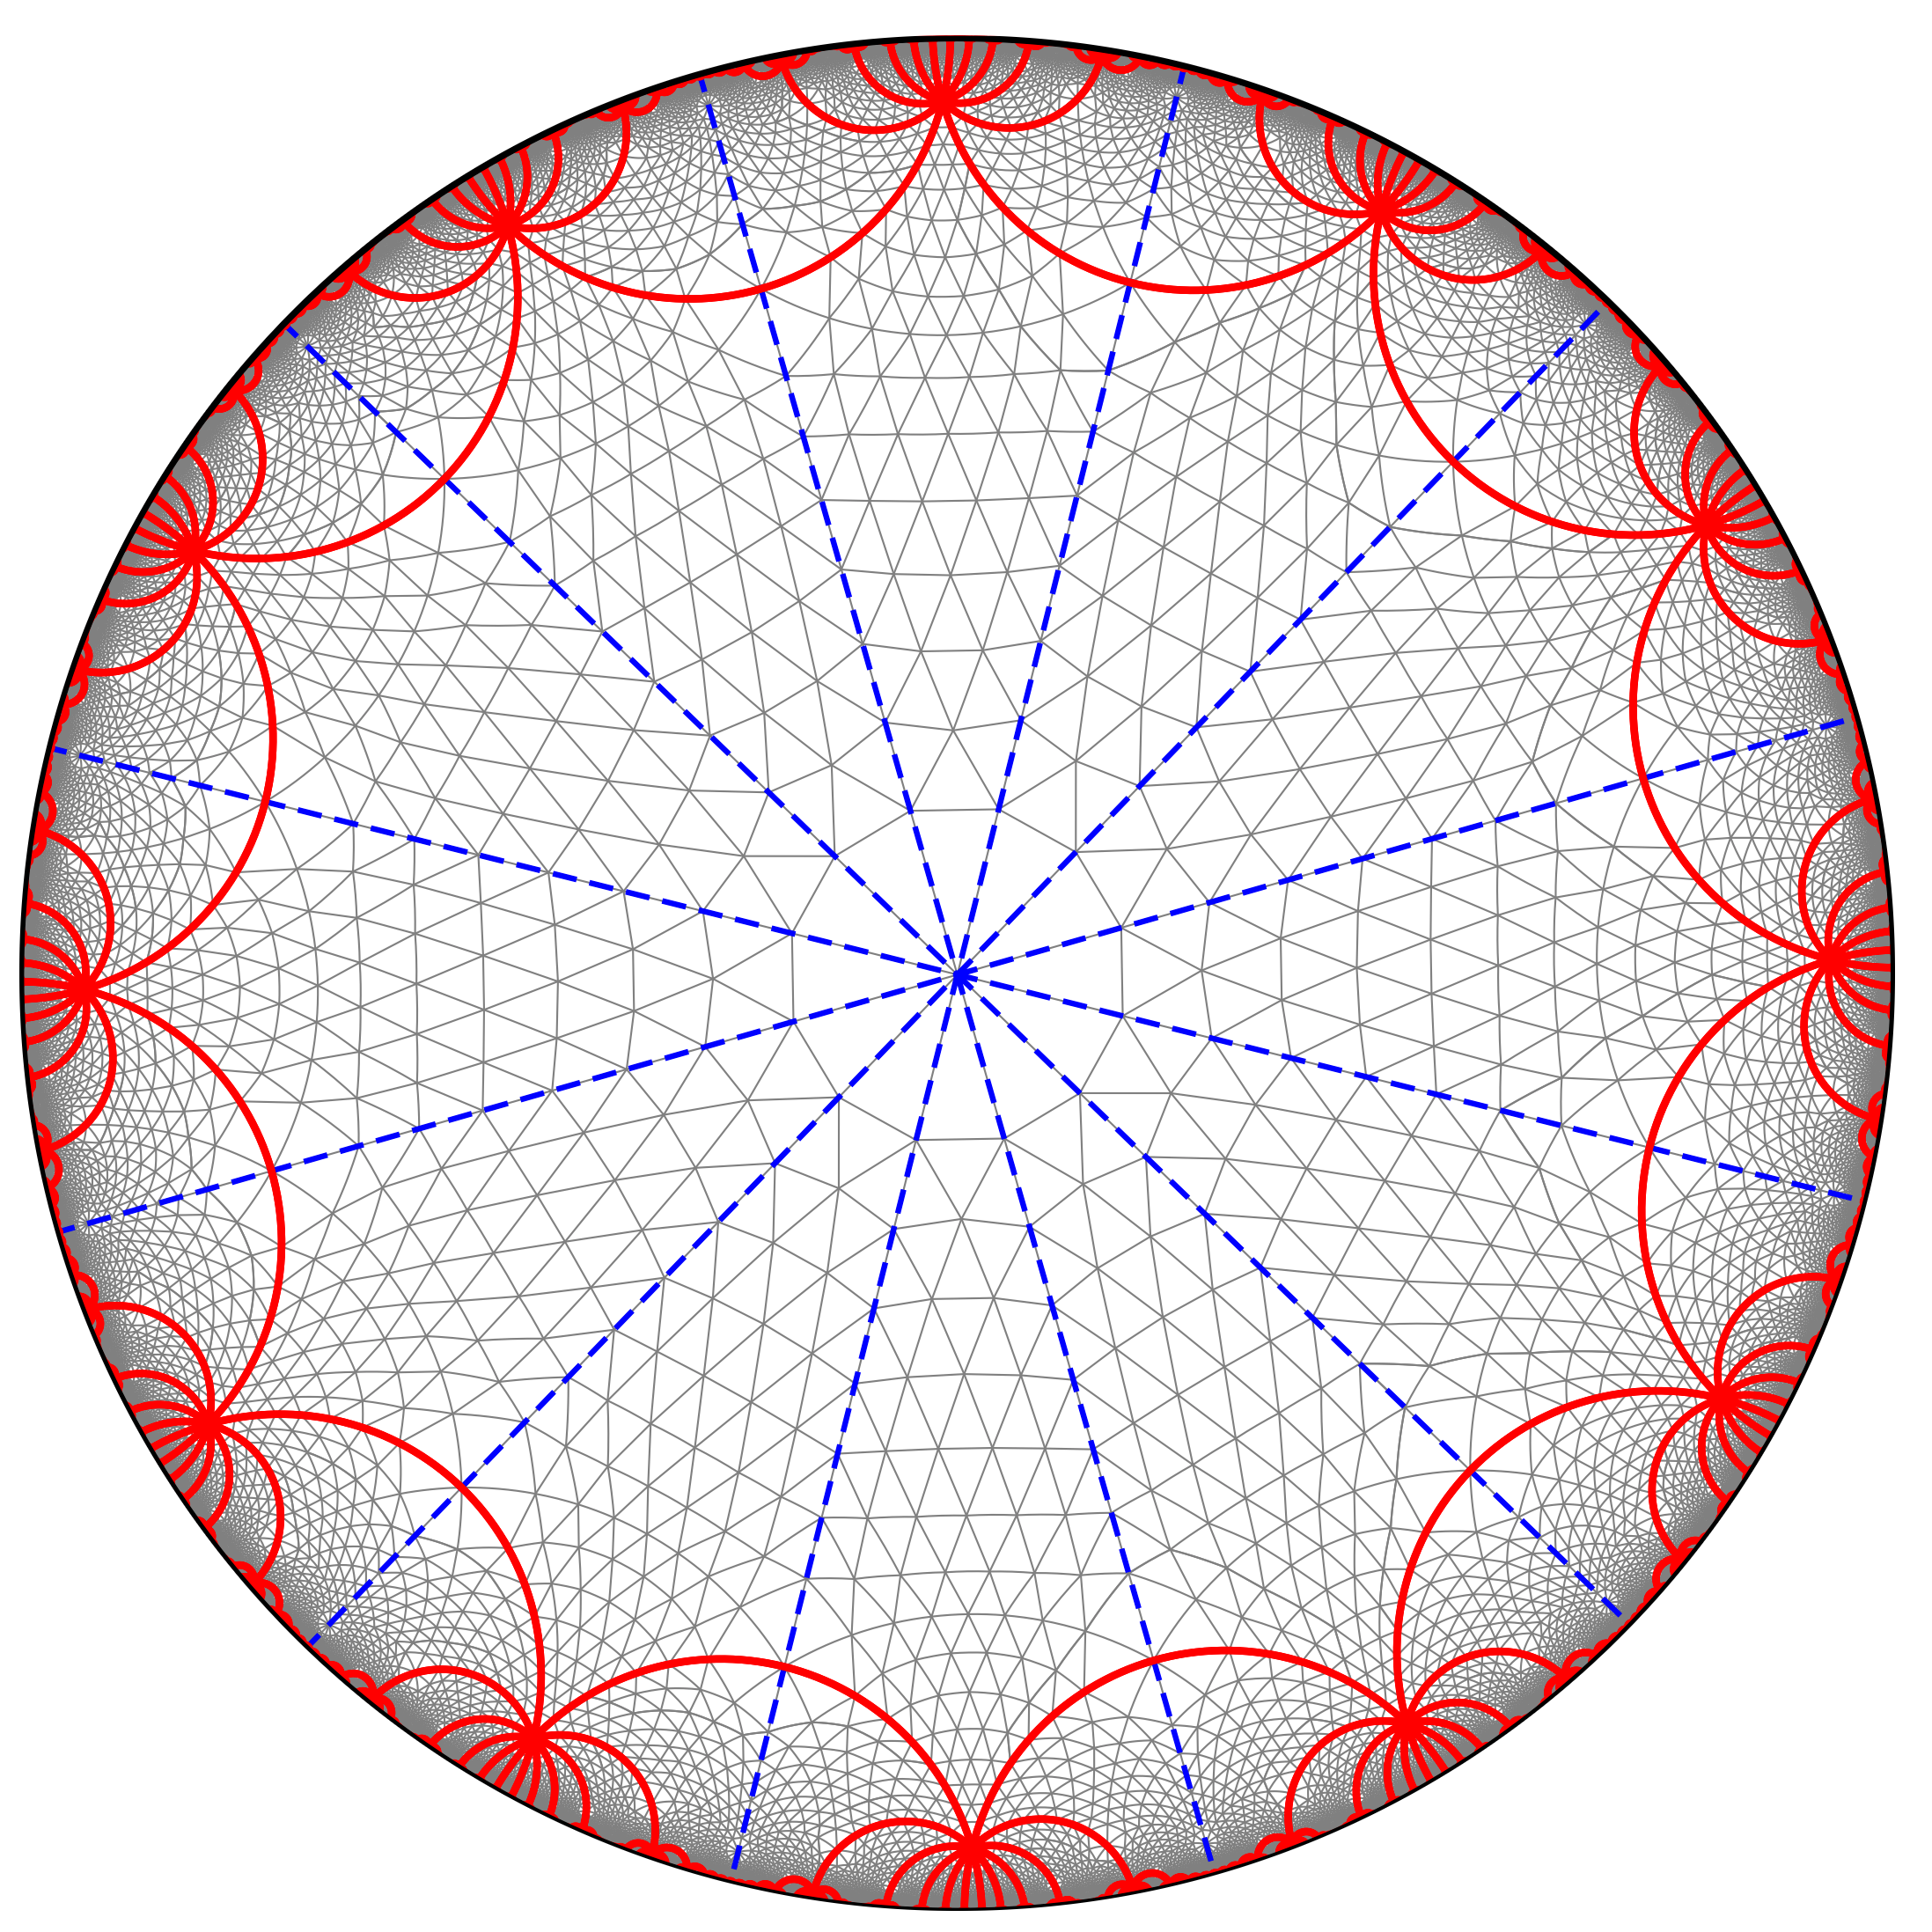
\includegraphics[width=\linewidth]{data/g3_hyperelliptic01/cover05.png}
\caption{Uniformization of Surface~\ref{eq:regular_hyperelliptic}. The surface admits
a regular fundamental polygon (red) with opposite sides identified. In this normalization
the axes of the identification motions meet in a point.}
\label{fig:regular_cover}
\end{figure}


\subsection{Weierstrass points on hyperelliptic surfaces}
A hyperelliptic surface comes together with a holomorphic involution $h$ called the hyperelliptic involution. The branch points are fixed points under this transformation. For a hyperelliptic algebraic curve it is $h(\mu, \lambda)=(-\mu, \lambda)$

\subsection{Canonical domains}
\subsection{The Wente torus}
\subsection{Lawsons surface}



\section{Schottky to Fuchsian Uniformization}

\begin{figure}
	\centering
	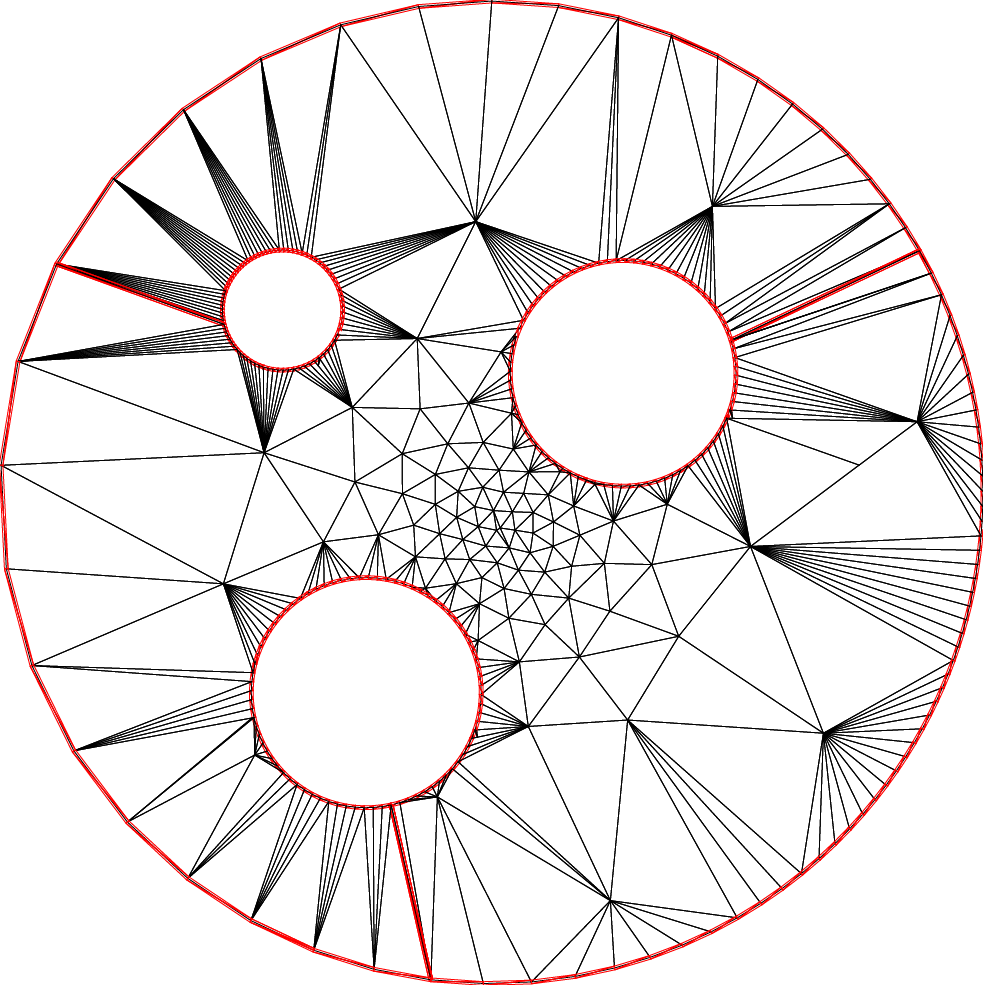
\includegraphics[width=0.45\linewidth]{data/g3_schottky01/schottky02_convert_pdf.png}
	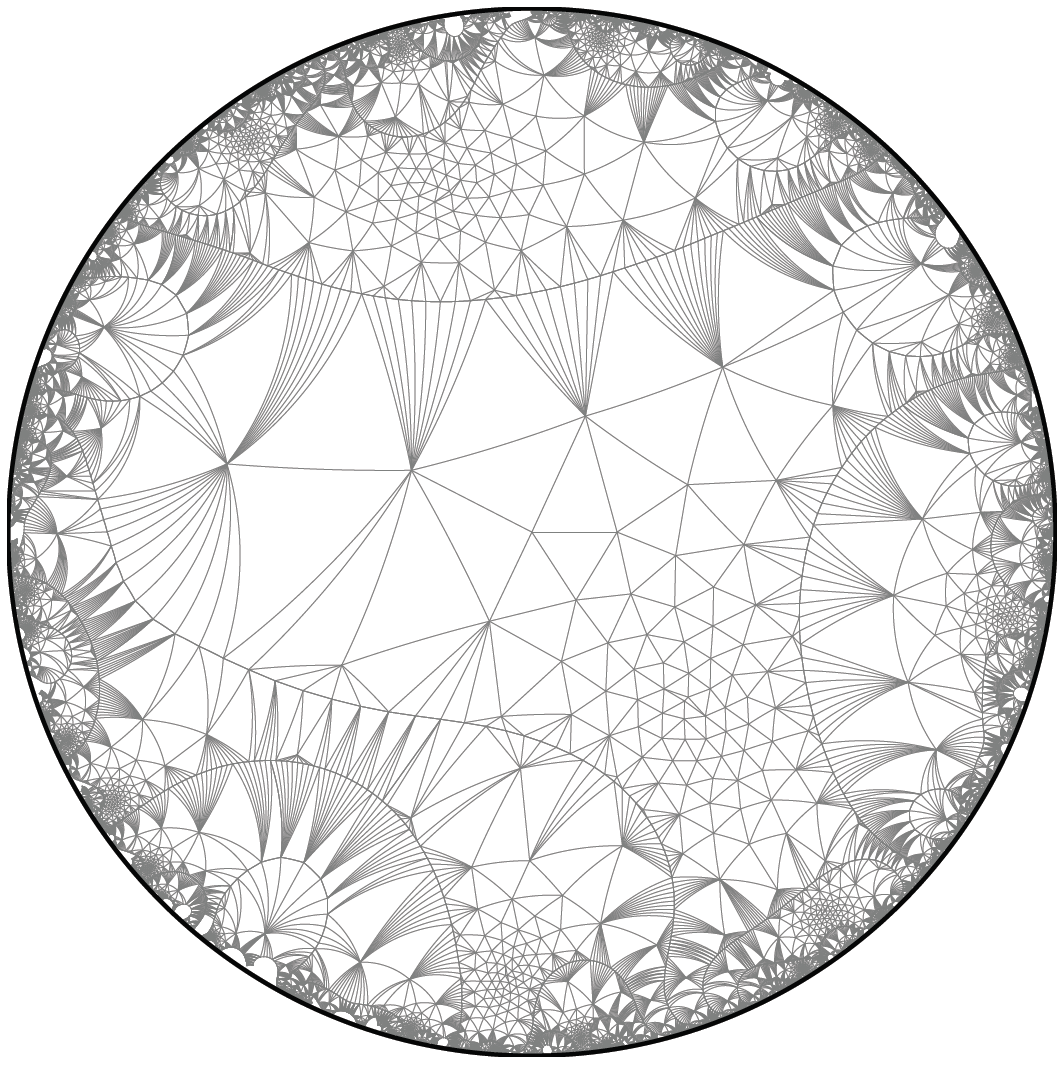
\includegraphics[width=0.45\linewidth]{data/g3_schottky01/schottky02_pdf.png}
	\caption{Fuchsian uniformization of a Riemann surface (right) given by Schottky data (left).}
	\label{fig:fuchsian_to_schottky}
\end{figure}

\begin{figure}
	\centering
	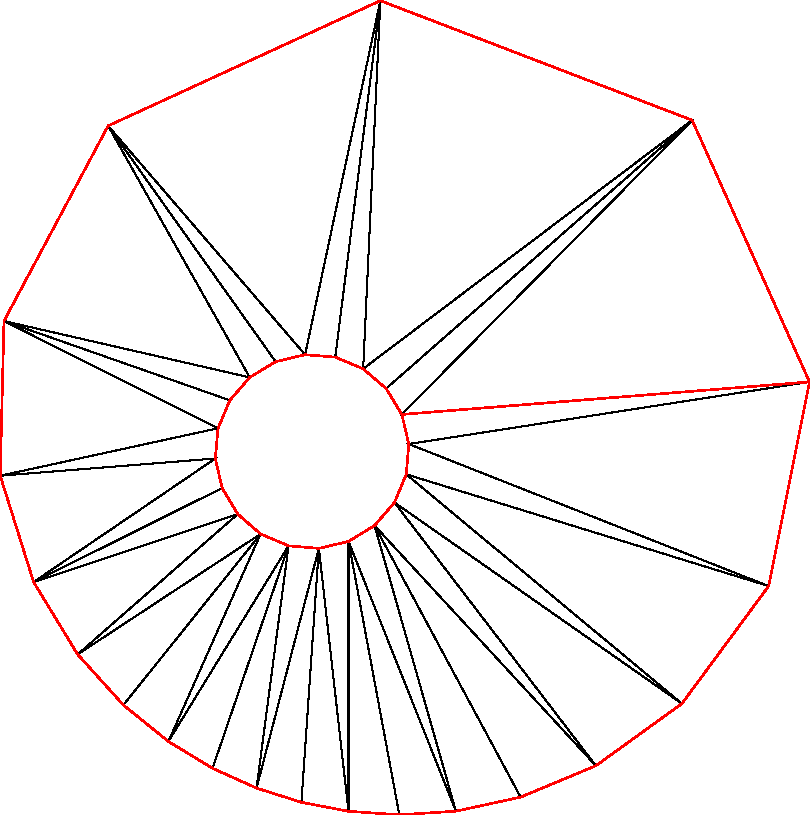
\includegraphics[width=0.3\linewidth]{image/schottky/g1_schottky_converted.pdf}
	\quad
	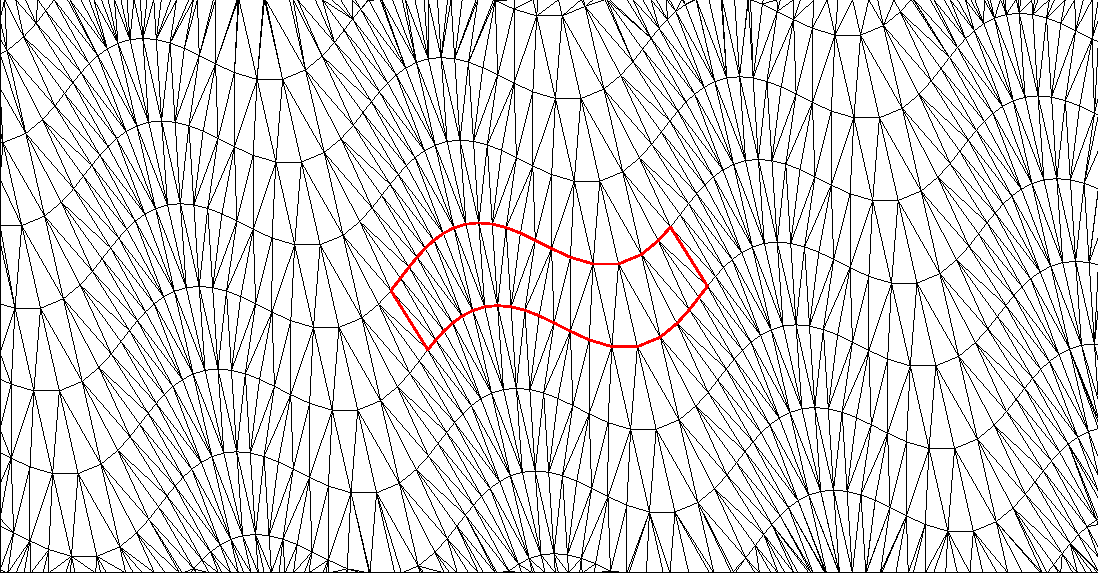
\includegraphics[width=0.6\linewidth]{image/schottky/g1_domain_converted.pdf}
	\caption{Uniformization of a genus $1$ discrete Riemann surface given by Schottky data.
	The boundary of the fundamental domain consists of circular polygons in the Schottky domain.}
	\label{fig:fuchsian_to_schottky_genus_1}
\end{figure}

In this section we show how to use the discrete theory to calculate a Fuchsian uniformization of a Riemann surface 
given by Schottky data. For a triangulated fundametal domain of a Schottky group we show how to obtain a discretely
conformally equivalent triangulation either in the unit disk for genus greater that $1$ or in $\C$, see Figure~\ref{fig:fuchsian_to_schottky}. These triangulations build
a fundamental domain for the corresponding uniformizing Fuchsian or translation group of the given Riemann surface. We only consider classical Schottky groups here.

Let $C_1,C'_1\ldots,C_g,C'_g$ be disjoint circles in $\hat{\C}$. 
\begin{definition}
A classical Schottky group $G$ is a Kleinian group
with generators $\sigma_1,\ldots,\sigma_g$ satisfying
\[\frac{\sigma_i z - B_i}{\sigma_i z - A_i} = \mu_i \frac{z - B_i}{z - A_i}, \quad\quad\quad 0 < \left|\mu_i\right|<1,\]
where $\sigma_i$ maps the exterior of $C_i$ onto the interior of $C'_i$. The points $A_i$ and $B_i$ lie inside the circles $C_i$ and $C'_i$ respectively \cite{bobenko2011riemann}. 
\end{definition}
Figure~\ref{fig:schottky_group} illustrates this construction.
The quotient space $\Chat/G$ is a Riemann surface of genus $g$. The group $G$ is called the uniformizing
Schottky group. The points $A_i,\ldots,A_g$ and $B_i,\ldots,B_g$ are fixed points of this map.
A generator $\sigma$ with parameters $A$, $B$ and $\mu$ is a loxodromic transformation with matrix representation 
\[
\sigma = \frac{1}{A-B}
\begin{pmatrix}
	A\sqrt{\mu}-\frac{B}{\sqrt\mu} & AB\left(\frac{1}{\sqrt\mu}-\sqrt{\mu}\right) \\
	\sqrt\mu-\frac{1}{\sqrt\mu} & \frac{A}{\sqrt\mu}-B\sqrt\mu
\end{pmatrix}.
\]

\begin{figure}
	\centering
	\scalebox{1.0}{\input{figures/schottky2.pdf_t}}
	\caption{Schottky group generating a Riemann surface of genus $2$. The point at infinity is not contained in 
any of the circles. The parameters $A$ and $B$ lie inside the cirlces by definition.}
	\label{fig:schottky_group}
\end{figure}



\subsection{Discretization}
Given a Riemann surface of genus $g$ and a classical Schottky uniformization, we calculate a corresponding 
Fuchsian uniformization using discrete conformal equivalence of spherical and hyperbolic triangle meshes.
A fundamental domain of the Schottky uniformization is the Riemann sphere without the interior of the circles.
We start with a classical Schottky group $G$. Let $\sigma_1,\ldots,\sigma_g$ be the generators of $G$. We choose circles around the fixed points of the

The triangulation of a fundamental domain has to respect the mappings between the circles. Vertices on identified 
circles have to be identified as well. It is however not clear a priori what the conformal structure of a triagulated 
fundamental domain is. The edge length on identified circles differ since there is a M{\" o}bius transformation 
between them. 

The idea to define the conformal structure is to use length cross-ratios instead of edge lengths. Both definitions are equivalent and define the conformal structure of a discrete Riemann surface. So given length cross ratios on edges we can calculate representative edge lengths in the discrete conformal class of the surface and, more obvious, vice versa. On boundary edges of the fundamental domain the length cross ratios agree since length-cross ratios are M{\" o}bius invariant.




\subsection{Images of isometric circles}
\subsection{Hyperelliptic data}

\section{Conformal maps to $\Chat$}
\subsection{Selection of Branch Data}
\subsection{Examples}

\section{Surfaces with boundary}
\label{sec:surfaces_with_boundary}
\subsection{Variation of edge length}
\subsection{Examples}
\begin{figure}
\centering
\resizebox{\textwidth}{!}{
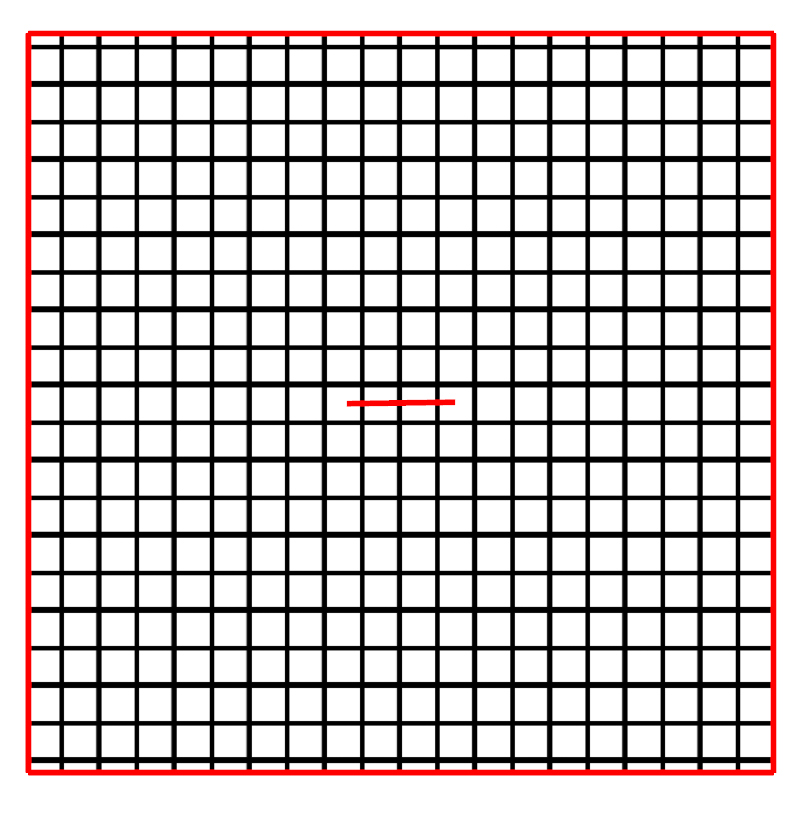
\includegraphics[width=0.5\linewidth]{image/slit_domain/domain_grid.png}
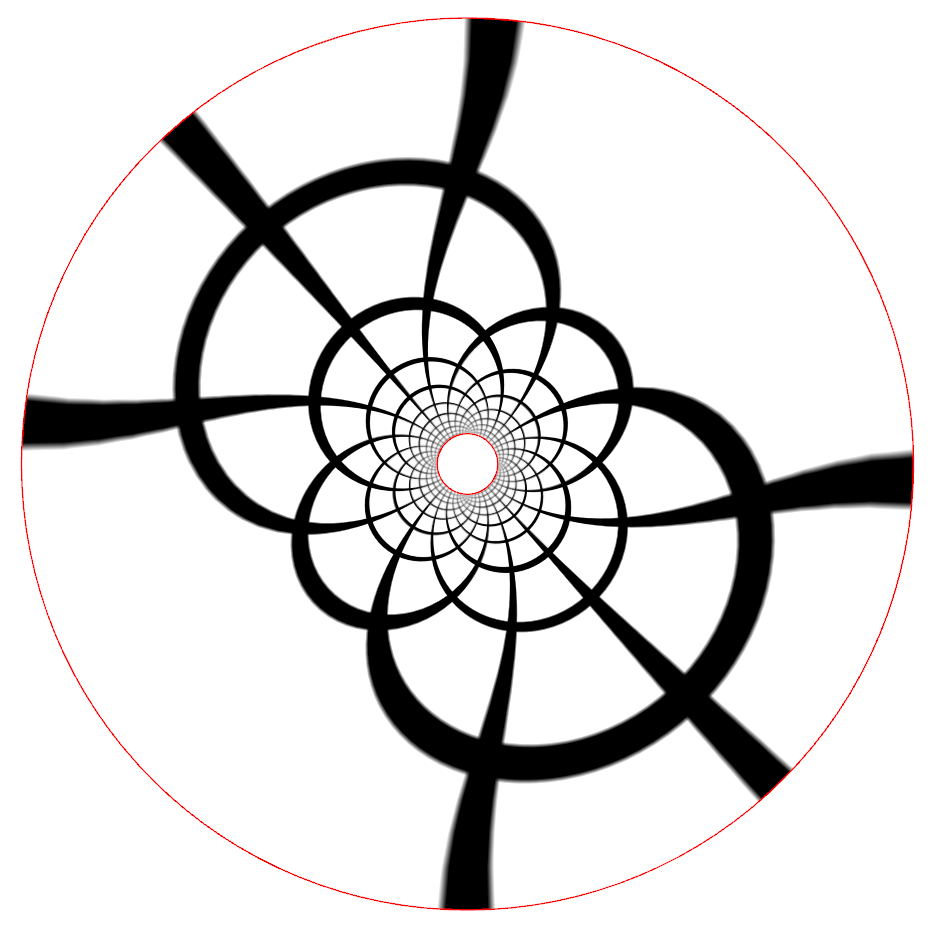
\includegraphics[width=0.5\linewidth]{image/slit_domain/image_grid.png}
}
\caption{Square with symmetric slit to the circle}
\label{fig:slit_circle}
\end{figure}


\section{Conformal maps of planar domains}
\label{sec:planar_domains}
\subsection{Boundary conditions}
\subsection{Comparison with examples of the Schwarz-Christoffel community}

\subfilebibliography
\end{document}

%%% Local Variables:
%%% TeX-master: "Thesis.tex"
%%% End: